\documentclass{beamer}
\usepackage{filecontents}



%construct dynamic page
\setbeamercovered{highly dynamic}
\newcounter{saveenumi}
\newcommand{\seti}{\setcounter{saveenumi}{\value{enumi}}}
\newcommand{\conti}{\setcounter{enumi}{\value{saveenumi}}}
\resetcounteronoverlays{saveenumi}

%set color and initial
\usetheme[progressbar=frametitle]{metropolis}
\definecolor{mygreen}{rgb}{.125,.5,.25}
\usecolortheme[named=mygreen]{structure}
\setbeamertemplate{frame numbering}[fraction]
\useoutertheme{metropolis}
\useinnertheme{metropolis}
\usefonttheme{metropolis}
\usecolortheme{spruce}
\setbeamercolor{background canvas}{bg=white}

\title{Bayesian Belief Networks}
\subtitle{with Graph Nueral Network}
\author{Phiphat Chomchit}
\institute{Chiang Mai University}

\begin{document}
	% Fill color in block
	\metroset{block=fill}
	
	\begin{frame}
		\titlepage
	\end{frame}

	\begin{frame}[t]{Source}
		\href{https://towardsdatascience.com/bbn-bayesian-belief-networks-how-to-build-them-effectively-in-python-6b7f93435bba}{BBN: Bayesian Belief Networks.\\ How to Build Them Effectively in Python}
	\end{frame}

	\begin{frame}[t]{Contents}
		\begin{itemize}
			\item The category of algorithms Bayesian Belief Networks (BBN) belong to
			\item Introduction to Bayesian Belief Networks (BBN) and Directed Acyclic Graphs (DAG)
			\item Bayesian Belief Network Python example using real-life data
			\item Conclusions
		\end{itemize}
	\end{frame}

	\begin{frame}[t]{What category of algorithms does Bayesian Belief Networks.}
		Technically there is no training happening within BBN. We simply define how different nodes in the network are linked together. Then we observe how the probabilities change after passing some evidence into certain nodes. Hence, I have put \textbf{Probabilistic Graphical Models} into their own category (see below).
		\begin{figure}
			\centering
			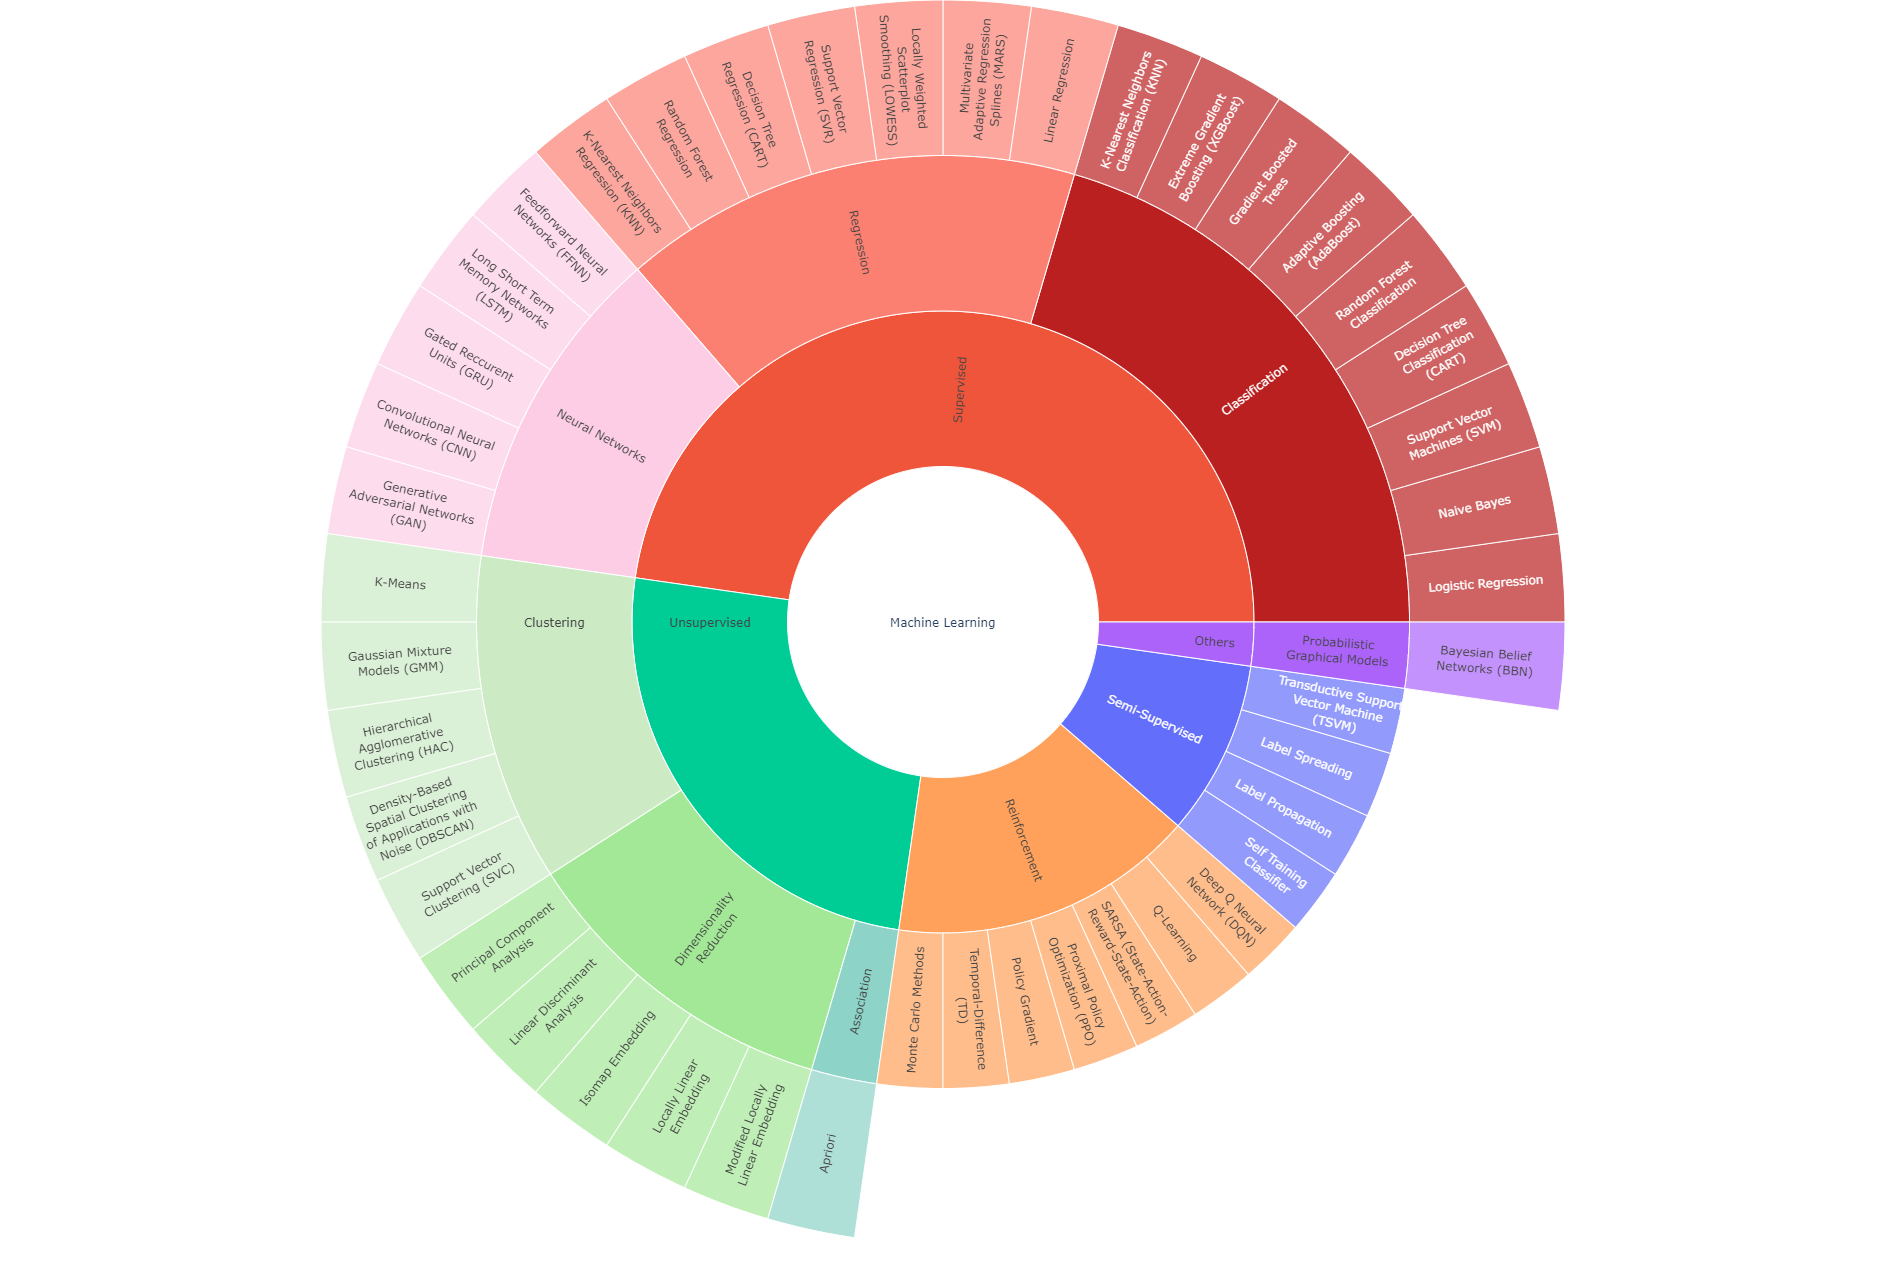
\includegraphics[scale=0.1]{newplot.png}
			\caption{Machine Learning Model}
		\end{figure}
	\end{frame}

	\begin{frame}[t]{Bayesian Belief Networks and Directed Acyclic Graphs(1/2)}
		Bayesian Belief Network (BBN) is a Probabilistic Graphical Model (PGM) that represents a set of variables and their conditional dependencies via a Directed Acyclic Graph (DAG).
		\begin{figure}
			\centering
			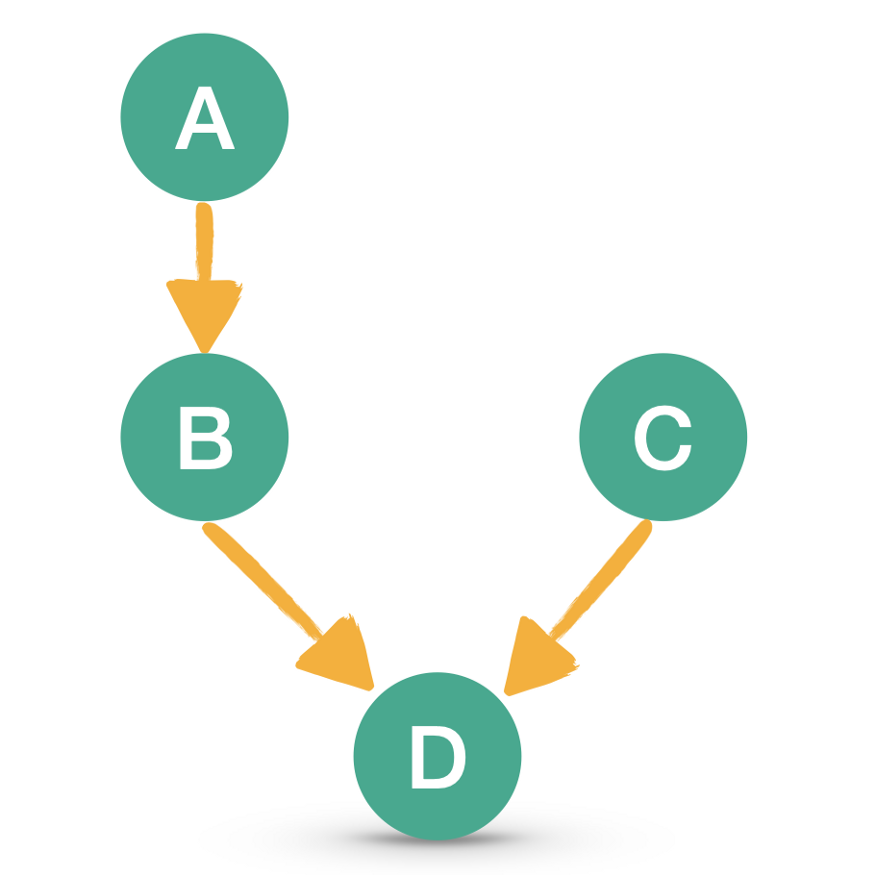
\includegraphics[scale=0.1]{dag.png}
			\caption{Directed Acyclic Graphs (Direction + No Loop)}
		\end{figure}
	\end{frame}

	\begin{frame}[t]{Bayesian Belief Networks and Directed Acyclic Graphs(2/2)}
	
		\begin{figure}
			\centering
			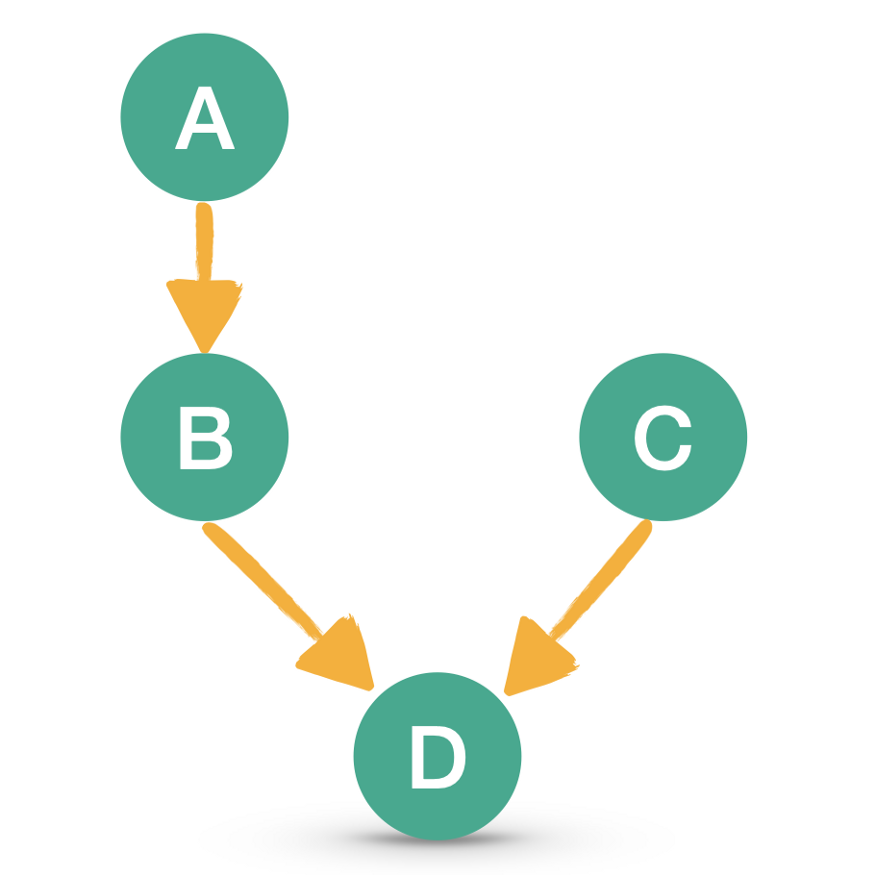
\includegraphics[scale=0.1]{dag.png}
			
		\end{figure}
		\begin{itemize}
			\item \textbf{Independence:}  A and C are independent of each other.
			\item \textbf{Dependence:} B is dependent on A since A is the parent of B.
			$$P(B | A)$$
			\item \textbf{Conditional Independence:} D is considered conditionally independent of A.
			$$P(D | B, A) = P(D | B)$$
		\end{itemize}
	\end{frame}

	\begin{frame}[t]{Directed Acyclic Graph for weather prediction}
		Let’s use Australian weather data to build a BBN. This will enable us to predict if it will rain tomorrow based on a few weather observations from today.
			\begin{figure}
			\centering
			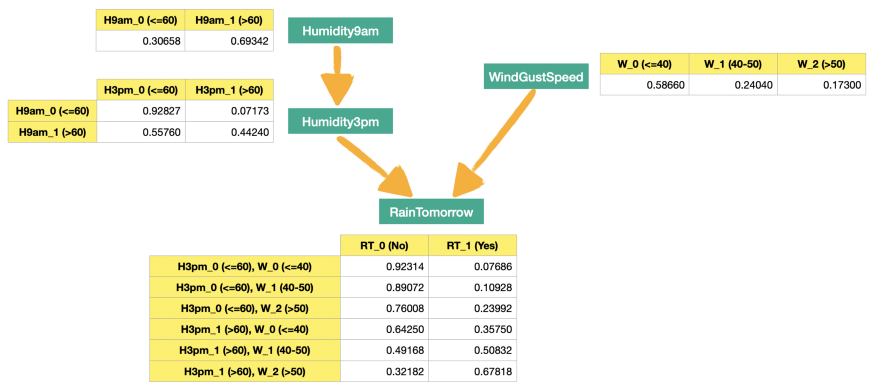
\includegraphics[scale=0.3]{bbn.png}
			\caption{Directed Acyclic Graph (DAG) for a Bayesian Belief Network (BBN) to forecast whether it will rain tomorrow.}
		\end{figure}
	\end{frame}
	
	\begin{frame}
		\begin{center}
			\Huge Code
		\end{center}
	\end{frame}

	\begin{frame}[standout]
		Q/A
	\end{frame}
\end{document}